\let\negmedspace\undefined
\let\negthickspace\undefined
\documentclass[journal]{IEEEtran}
\usepackage[a5paper, margin=10mm, onecolumn]{geometry}
\usepackage{tfrupee}
\setlength{\headheight}{1cm}
\setlength{\headsep}{0mm}
\usepackage{gvv-book}
\usepackage{gvv}
\usepackage{cite}
\usepackage{amsmath,amssymb,amsfonts,amsthm}
\usepackage{algorithmic}
\usepackage{graphicx}
\usepackage{float}
\usepackage{textcomp}
\usepackage{xcolor}
\usepackage{caption}
\usepackage{txfonts}
\usepackage{listings}
\usepackage{enumitem}
\usepackage{mathtools}
\usepackage{gensymb}
\usepackage{comment}
\usepackage[breaklinks=true]{hyperref}
\usepackage{tkz-euclide}
\usepackage{listings}
% \usepackage{gvv}
\def\inputGnumericTable{}
\usepackage[latin1]{inputenc}
\usepackage{color}
\usepackage{array}
\usepackage{longtable}
\usepackage{calc}
\usepackage{multirow}
\usepackage{hhline}
\usepackage{ifthen}
\usepackage{lscape}
\usepackage{tikz}
\usetikzlibrary{patterns}
\begin{document}
\bibliographystyle{IEEEtran}
\vspace{3cm}
\title{GATE 2024 MN }
\author{ai25btech11039
- Harichandana Varanasi}
\maketitle
% \maketitle
% \newpage
% \bigskip
{\let\newpage\relax\maketitle}
% \maketitle
% \newpage
% \bigskip
{\let\newpage\relax\maketitle}
\renewcommand{\thefigure}{\theenumi}
\renewcommand{\thetable}{\theenumi}
\setlength{\intextsep}{10pt} % Space between text and floats
\noindent\underline{\textbf{General Aptitude}}\\[0.5em] 
\noindent\textbf{Q.1 -- Q.5 carry one mark each.}
\vspace{0.5em}
\begin{enumerate}[leftmargin=0pt]
% Q1
\item If `$\to$' denotes increasing order of intensity, then the meaning of the words [drizzle $\to$ rain $\to$ downpour] is analogous to [ \underline{\hspace{1.5cm}} $\to$ quarrel $\to$ feud]. Which one of the given options is appropriate to fill the blank?
\begin{enumerate}
\begin{multicols}{4}
\item bicker
\item bog
\item dither
\item dodge
\end{multicols}
\end{enumerate}
\hfill{\brak{\text{GATE MN 2024}}}
% Q2
\item Statements:\\[0.5em]

1.All heroes are winners.\\
2.All winners are lucky people.\\

Inferences:\\
I. All lucky people are heroes.\\
II. Some lucky people are heroes.\\
III. Some winners are heroes.\\[0.5em]
Which of the above inferences can be logically deduced from statements 1 and 2?
\begin{enumerate}
\begin{multicols}{4}
\item Only I and II
\item Only II and III
\item Only I and III
\item Only III
\end{multicols}
\end{enumerate}
\hfill{\brak{\text{GATE MN 2024}}}
% Q3
\item A student was supposed to multiply a positive real number $p$ with another positive real number $q$. Instead, the student divided $p$ by $q$. If the percentage error in the \text{student's} answer is 80\%, the value of $q$ is
\begin{enumerate}
\begin{multicols}{4}
\item 5
\item $\sqrt{2}$
\item 2
\item $\sqrt{5}$
\end{multicols}
\end{enumerate}
\hfill{\brak{\text{GATE MN 2024}}}
% Q4
\item If the sum of the first 20 consecutive positive odd numbers is divided by $20^2$, the result is
\begin{enumerate}
\begin{multicols}{4}
\item 1
\item 20
\item 2
\item 1/2
\end{multicols}
\end{enumerate}
\hfill{\brak{\text{GATE MN 2024}}}
% Q5
\item The ratio of the number of girls to boys in class VIII is the same as the ratio of the number of boys to girls in class IX. The total number of students (boys and girls) in classes VIII and IX is 450 and 360, respectively. If the number of girls in classes VIII and IX is the same, then the number of girls in each class is
\begin{enumerate}
\begin{multicols}{4}
\item 150
\item 200
\item 250
\item 175
\end{multicols}
\end{enumerate}
\hfill{\brak{\text{GATE MN 2024}}}\\[0.5em]
\noindent\textbf{Q.6 -- Q.10 carry two marks each.}\\[0.5em]
% Q6
\item In the given text, the blanks are numbered (i)--(iv). Select the best match for all the blanks. \\[0.5em]

Yoko Roi stands \underline{\hspace{1cm}} (i) as an author for standing \underline{\hspace{1cm}} (ii) as an honorary fellow, after she stood \underline{\hspace{1cm}} (iii) her writings that stand \underline{\hspace{1cm}} (iv) the freedom of speech. \\[1em]

\begin{enumerate}
\item (i) out \quad (ii) down \quad (iii) in \quad (iv) for
\item (i) down \quad (ii) out \quad (iii) by \quad (iv) in
\item (i) down \quad (ii) out \quad (iii) for \quad (iv) in
\item (i) out \quad (ii) down \quad (iii) by \quad (iv) for
\end{enumerate}

\hfill{\brak{\text{GATE MN 2024}}}\\[0.5em]

% Q7
\item Seven identical cylindrical chalk-sticks are fitted tightly in a cylindrical container. The length of the container is equal to the length of the chalk-sticks. The ratio of the occupied space to the empty space of the container is
\begin{figure}[h!]
\centering
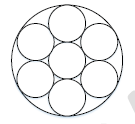
\includegraphics[width=0.5\linewidth]{figs/chalksticks.PNG}
\caption{Chalk sticks arrangement.}
\label{fig:chalk}
\end{figure}
\newpage
\begin{enumerate}
\item 5/2
\item 7/2
\item 9/2
\item 3
\end{enumerate}
\hfill{\brak{\text{GATE MN 2024}}}
% Q8
\item The plot below shows the relationship between the mortality risk of cardiovascular disease and the number of steps a person walks per day. Based on the data, which one of the following options is true?
\begin{figure}[h!]
\centering
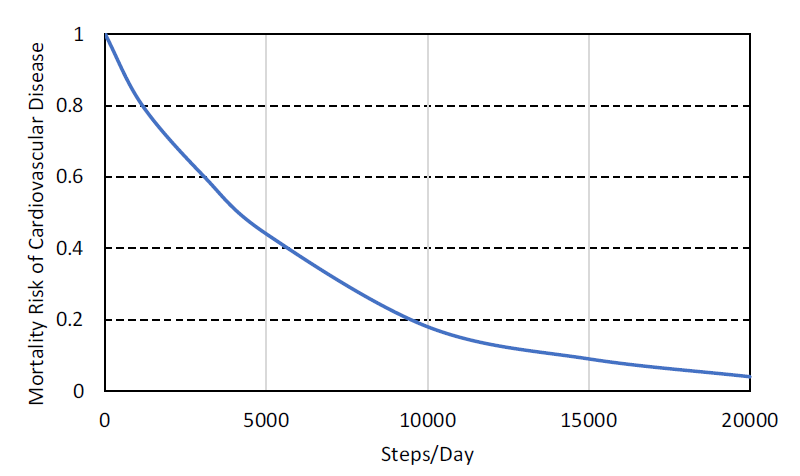
\includegraphics[width=0.5\linewidth]{figs/steps.PNG}
\caption{Mortality risk vs steps/day.}
\label{fig:mortality}
\end{figure}
\begin{enumerate}
\item The risk reduction on increasing the steps/day from 0 to 10000 is less than the risk reduction on increasing the steps/day from 10000 to 20000.
\item The risk reduction on increasing the steps/day from 0 to 5000 is less than the risk reduction on increasing the steps/day from 15000 to 20000.
\item For any 5000 increment in steps/day the largest risk reduction occurs on going from 0 to 5000.
\item For any 5000 increment in steps/day the largest risk reduction occurs on going from 15000 to 20000.
\end{enumerate}
\hfill{\brak{\text{GATE MN 2024}}}
% Q9
% Q9
\item Five cubes of identical size and another smaller cube are assembled as shown in Figure~\ref{fig:cubesA}. 
If viewed from direction X, the planar image of the assembly appears as Figure~\ref{fig:cubesB}. 
If viewed from direction Y, the planar image of the assembly (Figure~\ref{fig:cubesA}) will appear as:

\begin{figure}[h!]
    \centering
    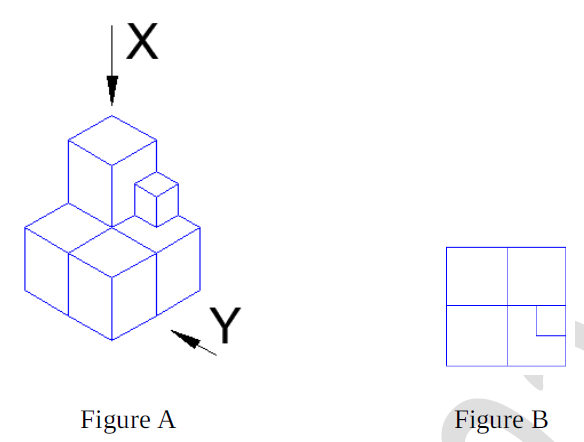
\includegraphics[width=0.35\linewidth]{figs/cubes.png}
    \caption{Assembly of cubes (Figures A and B).}
    \label{fig:cubesA}
\end{figure}

\begin{enumerate}
    \item \begin{minipage}[t]{0.8\linewidth}\raggedright
              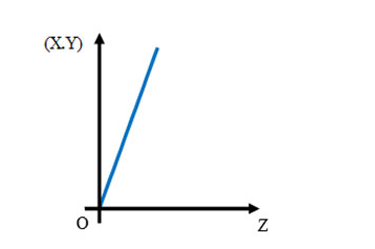
\includegraphics[width=0.25\linewidth]{figs/9a.png}\\
          \end{minipage}

    \item \begin{minipage}[t]{0.8\linewidth}\raggedright
              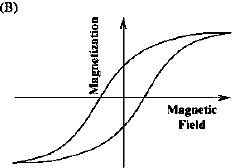
\includegraphics[width=0.25\linewidth]{figs/9b.png}\\
          \end{minipage}

    \item \begin{minipage}[t]{0.8\linewidth}\raggedright
              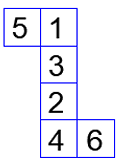
\includegraphics[width=0.25\linewidth]{figs/9c.png}\\
          \end{minipage}

    \item \begin{minipage}[t]{0.8\linewidth}\raggedright
              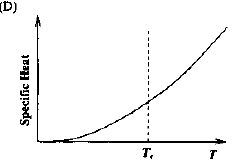
\includegraphics[width=0.25\linewidth]{figs/9d.png}\\
          \end{minipage}
\end{enumerate}

\hfill{\brak{\text{GATE MN 2024}}}


% Q10
\item Visualize a cube that is held with one of the four body diagonals aligned to the vertical axis. Rotate the cube about this axis such that its view remains unchanged. The magnitude of the minimum angle of rotation is
\begin{enumerate}
\item $120^\circ$
\item $60^\circ$
\item $90^\circ$
 \item 180\textdegree  % text degree


\end{enumerate}
\hfill{\brak{\text{GATE MN 2024}}}\\[0.5em]
\noindent\textbf{Q.11 -- Q.35 carry one mark each.}
% Q11
\item Exposure to loud impulsive noise may lead to
\begin{enumerate}
\begin{multicols}{4}
\item Nystagmus
\item Siderosis
\item Tinnitus
\item Stannosis
\end{multicols}
\end{enumerate}
\hfill{\brak{\text{GATE MN 2024}}}
\newpage
% Q12
\item In a self-contained closed-circuit breathing apparatus,
\begin{enumerate}
\item the exhaled air is released outside the apparatus.
\item the exhaled air is wholly absorbed within the apparatus.
\item CO$_2$ is released outside the apparatus after separating from exhaled air.
\item CO$_2$ from exhaled air is absorbed with a chemical.
\end{enumerate}
\hfill{\brak{\text{GATE MN 2024}}}
% Q13
\item A rectangular mine airway of 2.0 m width and 2.5 m height has a bend with deflection of $\pi$/2 radian. If the radius of curvature of the bend is 4.0 m, the shock factor of the bend is (round off to three decimals)
\begin{enumerate}
\item 0.014
\item 0.024
\item 0.051
\item 0.071
\end{enumerate}
\hfill{\brak{\text{GATE MN 2024}}}
% Q14
\item In an underground coal mine, two fatalities and three serious bodily injuries occurred during the year 2022. The average daily employment is 1100 and annual working days is 300. The severity index as per DGMS guideline for the mine is
\begin{enumerate}
\item 12.32
\item 25.58
\item 31.21
\item 34.63
\end{enumerate}
\hfill{\brak{\text{GATE MN 2024}}}
% Q15
\item For a geared engine winding system, the man winding cage is placed at its normal position at pit top of the shaft. As per CMR 2017, the minimum space, in m, between the center of the hole of the detaching hook attached to the rope shackle and detaching bell plate is
\begin{enumerate}
\item 3.6
\item 2.4
\item 1.8
\item 1.5
\end{enumerate}
\hfill{\brak{\text{GATE MN 2024}}}
% Q16
\item The value of integral, $I = \int_{0}^{\pi/4} \cos x \, \sin^{3}x \, dx$ is

\begin{enumerate}
    \item $\dfrac{1}{64}$\\[0.5em]
    \item $\dfrac{1}{16}$\\[0.5em]
    \item $\dfrac{1}{4}$\\[0.5em]
    \item $1$
\end{enumerate}

\hfill{\brak{\text{GATE MN 2024}}}
% Q17
\item The value of $\lim_{x \to 0} \left(\dfrac{n \sin 5x}{\sin 3x}\right)$ is

\begin{enumerate}
    \item $2n$\\[0.5em]
    \item $\dfrac{3n}{5}$\\[0.5em]
    \item $\dfrac{6n}{5}$\\[0.5em]
    \item $\dfrac{5n}{3}$\\[0.5em]
\end{enumerate}
\hfill{\brak{\text{GATE MN 2024}}}
% Q18
\item The spherical semivariogram model $\gamma(h)$ is represented by the following 
expression, where $h$ is the lag distance.
\[
\gamma(h) =
\begin{cases}
C_{0}, & \text{for } h = 0, \\[0.5em]
C_{0} + (C - C_{0})\left[1.5 \dfrac{h}{a} - 0.5 \left(\dfrac{h}{a}\right)^3 \right], & \text{for } 0 < h \leq a, \\[0.5em]
C, & \text{for } h > a
\end{cases}
\]

The parameters $C_{0}, C$ and $a$ are respectively known as

\begin{enumerate}[
    \item nugget, range and sill.
    \item sill, nugget and range.
    \item sill, range and nugget.
    \item nugget, sill and range.
\end{enumerate}

\hfill{\brak{\text{GATE MN 2024}}}
% Q19
\item In a M/M/1 system, the inter-arrival time of dumpers to a shovel follows exponential distribution with a mean arrival rate of 9 dumpers per hour. The service time of the shovel follows exponential distribution with a mean service rate of 12 dumpers per hour. The probability that exactly one dumper is available to the shovel is
\begin{enumerate}
\item 1/16
\item 3/16
\item 3/4
\item 1/4
\end{enumerate}
\hfill{\brak{\text{GATE MN 2024}}}
% Q20
\item A project network with the sequence of five activities is shown.

\begin{figure}[h!]
  \centering
  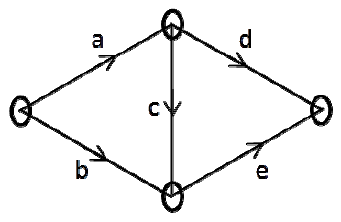
\includegraphics[width=0.5\linewidth]{figs/network.png}
  \label{fig:project}
\end{figure}
% Bring the table in exactly here (non-floating)
\begin{table}[h!]
  \centering
  \begin{tabular}{|c|c|c|c|c|c|}
    \hline
    Activity & A & B & C & D & E \\ \hline
    Duration (week) & 5 & 6 & 8 & 3 & 4 \\
    Crashing cost per week (lakh INR) & 4.0 & 2.5 & 2.0 & 3.0 & 4.0 \\ \hline
  \end{tabular}
  \caption{Activity durations and crashing costs}
  \label{tab:activities}
\end{table}

If the project is crashed by one week, the increase in project cost, in lakh INR, is
The crashing costs of activities are shown in Table~\ref{tab:activities}.
\begin{enumerate}
  \item 2.0
  \item 2.5
  \item 3.0
  \item 4.0
\end{enumerate}

\hfill{\brak{\text{GATE MN 2024}}}


% Q21
\item Match the following features with the corresponding symbols

% Pull the table from an external file (non-floating, numbered with caption)
\begin{center}
  \captionof{table}{Symbols and descriptions for matching}\label{tab:match}
  \begin{tabular}{|c|l|c|c|}
    \hline
    \textbf{Symbol} & \textbf{Description} & \textbf{Code} & \textbf{Figure} \\ \hline
    P & Shaft                    & 1 & 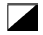
\includegraphics[width=0.10\linewidth]{figs/21a.png} \\ 
    Q & Staple shaft             & 2 & 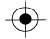
\includegraphics[width=0.10\linewidth]{figs/21b.png} \\ 
    R & Abandoned shaft          & 3 & 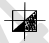
\includegraphics[width=0.10\linewidth]{figs/21c.png} \\ 
    S & Abandoned staple shaft   & 4 & 
\includegraphics[width=0.10\linewidth]{figs/21d.png} \\ \hline
  \end{tabular}
\end{center}


\begin{enumerate}
\item P$\to$1; Q$\to$3; R$\to$4; S$\to$2\\[0.5em]
\item P$\to$4; Q$\to$2; R$\to$1; S$\to$3\\[0.5em]
\item P$\to$2; Q$\to$4; R$\to$3; S$\to$1\\[0.5em]
\item P$\to$4; Q$\to$1; R$\to$2; S$\to$3\\[0.5em]
\end{enumerate}
\hfill{\brak{\text{GATE MN 2024}}}

% Q22
\item If the major ($\sigma_1$) and minor ($\sigma_3$) principal stresses for a rock element have a relationship as $\sigma_3 = -\frac{1}{2} \sigma_1$, the maximum shear stress is expressed by
\begin{enumerate}
\item $\frac{3}{4}\sigma_1$\\[0.5em]
\item $\frac{4}{3}\sigma_1$\\[0.5em]
\item $\frac{1}{2}\sigma_1$\\[0.5em]
\item $\frac{1}{3}\sigma_1$\\[0.5em]
\end{enumerate}
\hfill{\brak{\text{GATE MN 2024}}}
% Q23
\item The ore that is NOT used for commercial extraction of metal is
\begin{enumerate}
\item Wolframite.
\item Dolomite.
\item Cassiterite.
\item Uraninite.
\end{enumerate}
\hfill{\brak{\text{GATE MN 2024}}}
% Q24
\item The function of District Mineral Foundation established by state governments in India, is to
\begin{enumerate}
\item look after safety aspects of mining operations.
\item approve mining plan.
\item act as an environmental regulatory body.
\item monitor welfare of mining affected people.
\end{enumerate}
\hfill{\brak{\text{GATE MN 2024}}}
% Q25
\item The percentage Fe and corresponding net value for an iron ore mine is given below
(Table~\ref{tab:fe-values}).

\begin{center}
  \captionof{table}{Fe percentage and net value}\label{tab:fe-values}
  \begin{tabular}{|c|c|}
    \hline
    \textbf{Fe (\%)} & \textbf{Net value (INR per tonne)} \\ \hline
    58 & 4000 \\ \hline
    62 & 4500 \\ \hline
  \end{tabular}
\end{center}
 % non-floating table inserted exactly here

Assuming net value versus grade curve to be a straight line, and mining cost of waste is
INR 1000 m$^3$, the correct representation of stripping ratio, $SR$ (m$^3$/tonne) versus Fe (\%) grade curve is

\begin{enumerate}
    \item $SR = -3.250 + 0.125\times \mathrm{Fe}$
    \item $SR = \;\;3.250 + 0.125\times \mathrm{Fe}$
    \item $SR = \;\;3250 + 125\times \mathrm{Fe}$
    \item $SR = -3250 + 125\times \mathrm{Fe}$
\end{enumerate}

\hfill{\brak{\text{GATE MN 2024}}}


\hfill{\brak{\text{GATE MN 2024}}}
% Q26
\item The magnitude of the curl of the vector $V = 2x i + 3y j + 4z k$, is
\begin{enumerate}
\item 0
\item 4
\item 9
\item 25
\end{enumerate}
\hfill{\brak{\text{GATE MN 2024}}}
% Q27
\item An explosive with a density of 1.2 g/cm$^3$ has a heat of explosion equal to 900 cal/g. If the heat of explosion of ANFO with density of 0.8 g/cm$^3$ is 950 cal/g, the bulk strength of the explosive relative to ANFO is \underline{\hspace{1.5cm}}. (round off up to 2 decimals)
\hfill{\brak{\text{GATE MN 2024}}}
% Q28
\item A typical 24-hour activity of a mobile crusher plant is shown. The utilization, in %, of the plant, is \underline{\hspace{1.5cm}}. (round off up to 2 decimals)
\begin{figure}[h!]
\centering
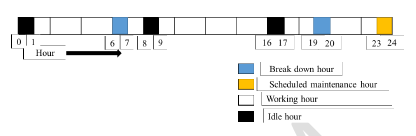
\includegraphics[width=0.5\linewidth]{figs/mobilecrusher.png}
\caption{24-hour activity.}
\label{fig:activity}
\end{figure}
\hfill{\brak{\text{GATE MN 2024}}}
% Q29
\item Polluted air with particulate matters of diameter 50 $\mu$m enter with a horizontal velocity of 1.0 m/s at a height of 0.5 m from the bottom of a dry settling chamber. The density of the particle is 2000 kg/m$^3$ and dynamic viscosity of the air is $1.8 \times 10^{-5}$ kg/(m·s). Assume streamline flow and the density of air is negligible as compared to particles and uniform horizontal velocity of 1.0 m/s of gas and particles within the chamber. Considering particle settling follows \textit{Stokes'} law, the minimum length in m, of the chamber required for settling of the particle at its bottom, is \underline{\hspace{1.5cm}}. (round off up to 2 decimals)

\hfill{\brak{\text{GATE MN 2024}}}
% Q30
\item The combined sound pressure level measured at a point in a production bench due to one dumper and one shovel is 95 dB(A). If the sound pressure level of shovel alone is 90 dB(A), the sound pressure level of the dumper alone, in dB(A), at the same point is \underline{\hspace{1.5cm}}. (round off up to 2 decimals)
\hfill{\brak{\text{GATE MN 2024}}}
% Q31
\item The void ratio of an unconsolidated soil heap of volume 1000 m$^3$ is 1.0. If the soil heap is consolidated to a volume of 800 m$^3$, the corresponding void ratio is \underline{\hspace{1.5cm}}. (round off up to 2 decimals)
\hfill{\brak{\text{GATE MN 2024}}}
% Q32
\item For a circular path of radius 300 m, the super elevation is restricted to 0.1 m for a width of 1.6 m. The maximum speed, in m/s, of vehicle to avoid overturn is \underline{\hspace{1.5cm}}. (round off up to 2 decimals)
\hfill{\brak{\text{GATE MN 2024}}}
% Q33
\item A scanline survey between points A and B of a rock mass is shown. Consider $RQD = 100 \times (0.1 + (0.1 \lambda) + (0.1 \lambda)^2 + \dots)$, where, $\lambda$ is the frequency of discontinuity per m. The RQD of the rock mass is \underline{\hspace{1.5cm}}. (round off up to 2 decimals)
\begin{figure}[h!]
\centering
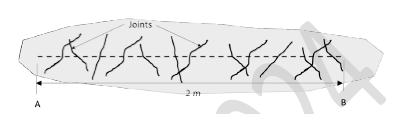
\includegraphics[width=0.5\linewidth]{figs/scanlinesurvey.png}
\caption{Scanline survey.}
\label{fig:scanline}
\end{figure}
\hfill{\brak{\text{GATE MN 2024}}}
% Q34
\item In a VCR stope, blast holes of 165 mm diameter are drilled. For the blast hole to behave as a spherical charge, the maximum charge length, in m, is \underline{\hspace{1.5cm}}. (round off up to 2 decimals)
\hfill{\brak{\text{GATE MN 2024}}}
% Q35
\item A rectangular development heading of dimension 3 m $\times$ 2.8 m is to be blasted with holes of 2.4 m in length. If the pull factor is 0.95 and swell factor is 1.20, the volume of blasted rock per round, in m$^3$, is \underline{\hspace{1.5cm}}. (round off up to 2 decimals)
\hfill{\brak{\text{GATE MN 2024}}}
\noindent\textbf{Q.36 -- Q.65 carry two marks each.}
% Q36
\item Data from two production faces of an open pit iron ore mine are given
(Table~\ref{tab:faces-data}).

\begin{center}
  \captionof{table}{Face-wise data for production planning}\label{tab:faces-data}
  \begin{tabular}{|l|c|c|}
    \hline
    \textbf{Item description} & \textbf{Face 1} & \textbf{Face 2} \\ \hline
    Maximum production capacity (tonne/day) & 1600 & 2000 \\ \hline
    Fe (\%) & 63 & 58 \\ \hline
    Production cost of ores (in INR/tonne) & 1500 & 1200 \\ \hline
  \end{tabular}
\end{center}
  % inserts the table exactly here (non-floating)

Ores from two different faces are blended and supplied with Fe grade not less than 60\%.
Based on the demand, the combined production is limited to a maximum of 2500 tonne/day.
If the selling price of blended iron ore is INR 4500/tonne, the optimal production from
two faces in tonne/day, for maximizing the profit, respectively are

\begin{enumerate}
  \item 1000.0 and 1500.0
  \item 1333.3 and 1166.7
  \item 1600.0 and 900.0
  \item 500.0 and 2000.0
\end{enumerate}

\hfill{\brak{\text{GATE MN 2024}}}

\hfill{\brak{\text{GATE MN 2024}}}
% Q37
\item Four identical districts of a mine are ventilated with a quantity of 3500 m$^3$/min at a fan drift pressure of 1.15 kPa. When one of the districts is sealed off, the change in resultant resistance is 0.072 Ns$^2$m$^{-8}$. If the fan is stopped, keeping a district sealed, the quantity through the mine becomes 850 m$^3$/min. The natural ventilation pressure in Pa, is
\begin{enumerate}
\item 72.12
\item 82.28
\item 105.56
\item 144.56
\end{enumerate}
\hfill{\brak{\text{GATE MN 2024}}}
% Q38
\item Matrix $A=\begin{bmatrix}1&4&3\\ 5&2&1\\ 6&4&3\end{bmatrix}$, and $B=A-A^{T}$, then $B$ is
\begin{enumerate}
\item symmetric.
\item skew symmetric.
\item diagonal.
\item scalar.
\end{enumerate}
\hfill{\brak{\text{GATE MN 2024}}}

% Q39
\item The roof convergence data for 30 days at a monitoring station in a coal mine gallery is given (Table~\ref{tab:q39-conv}).

\begin{center}
  \captionof{table}{Convergence readings over 30 days}\label{tab:q39-conv}
  \begin{tabular}{|c|c|}
    \hline
    \textbf{Day} & \textbf{Convergence reading (mm)} \\ \hline
     0 &  0.0  \\ \hline
     5 &  4.7  \\ \hline
    10 & 11.3  \\ \hline
    16 & 19.6  \\ \hline
    22 & 28.8  \\ \hline
    30 & 34.8  \\ \hline
  \end{tabular}
\end{center}
 % non-floating table inserted exactly here

The management decides on a Trigger Action Response Plan (TARP) if the following two premises occur simultaneously.\\[0.4em]
\textbf{Premise 1:} Rate of convergence exceeds 1.5 mm/day between two consecutive measurements.\\
\textbf{Premise 2:} Rate of cumulative increase in convergence exceeds 1.0 mm/day.\\[0.6em]
Identify the day on which TARP is enforced in that gallery.

\begin{enumerate}
  \item 10
  \item 16
  \item 22
  \item 30
\end{enumerate}

\hfill{\brak{\text{GATE MN 2024}}}

% Q40
\item Magnitude of error in the determination of the integral, I using \textit{Simpson's rule}
 1/3 rule, taking step length as 1.0 is
$I = \int_1^3 (x^3 + 6) dx$
\begin{enumerate}
\item 0
\item 1.0
\item 1.5
\item 2.0
\end{enumerate}
\hfill{\brak{\text{GATE MN 2024}}}
% Q41
\item In a closed traverse, ABC, the bearings of two lines AB and BC are given
(Table~\ref{tab:q41-bear}).

\begin{center}
  \begin{tabular}{|c|c|c|}
    \hline
    \textbf{Line} & \textbf{Length (m)} & \textbf{Bearing} \\ \hline
    AB & 100 & $90^\circ$ \\ 
    BC & 120 & $150^\circ$ \\ \hline
  \end{tabular}
\end{center}
 % inserts the table exactly here

The length, in m, and bearing of line CA, in degree, respectively, are

\begin{enumerate}
\item $190.7$ and $303^\circ$
\item $190.7$ and $240^\circ$
\item $160.3$ and $240^\circ$
\item $160.3$ and $303^\circ$
\end{enumerate}
\hfill{\brak{\text{GATE MN 2024}}}

\newpage
% Q42
\item Match the method of mining with orebody geometry, orebody strength and type of supports
(Table~\ref{tab:q42-match}).

\begin{center}
  \captionof{table}{Geometry, strength, support and method}\label{tab:q42-match}
  \setlength{\tabcolsep}{6pt}
  \renewcommand{\arraystretch}{1.15}
  \begin{tabular}{|l|l|l|l|}
    \hline
    \textbf{Geometry} & \textbf{Strength} & \textbf{Support} & \textbf{Method} \\ \hline
    % Each cell is its own mini-table (most reliable for multi-line cells)
    \begin{tabular}[t]{@{}l@{}}
      P.\ Tabular \& Moderately Steep\\
      Q.\ Tabular \& Flat\\
      R.\ Massive and Steep
    \end{tabular}
    &
    \begin{tabular}[t]{@{}l@{}}
      L.\ Strong\\
      M.\ Moderate\\
      N.\ Weak
    \end{tabular}
    &
    \begin{tabular}[t]{@{}l@{}}
      X.\ Unsupported\\
      Y.\ Artificially Supported\\
      Z.\ Self-supported
    \end{tabular}
    &
    \begin{tabular}[t]{@{}l@{}}
      1.\ Cut and Fill\\
      2.\ Block Caving\\
      3.\ Room and Pillar
    \end{tabular}
    \\ \hline
  \end{tabular}
\end{center}
 % draws the table exactly here

\begin{enumerate}
  \item P--L--Y--3; Q--N--Z--1; R--M--X--2
  \item P--M--Y--2; Q--N--Z--1; R--L--X--3
  \item P--L--Y--2; Q--M--Z--3; R--N--X--1
  \item P--L--Y--1; Q--L--Z--3; R--N--X--2
\end{enumerate}


\hfill{\brak{\text{GATE MN 2024}}}


% Q43
\item Vectors $\vec{a} = 2 \hat{i} + 3 \hat{j} - 4 \hat{k}$ and $\vec{b} = 4 \hat{i} + 2 \hat{j} + 3 \hat{k}$ represent the two adjacent sides of a triangle. The magnitude of the area of the triangle and the unit vector perpendicular to both $\vec{a}$ and $\vec{b}$ respectively, are
\begin{enumerate}
\item 28.93 and 0.581 - 0.76j - 0.27k
\item 28.93 and 17.01 - 22.0j - 8.0k
\item 14.46 and 0.581 - 0.76j - 0.27k
\item 14.46 and 17.01 - 22.0j - 8.0k
\end{enumerate}
\hfill{\brak{\text{GATE MN 2024}}}
% Q44
\item Water is pumped from a mine sump at the rate of 300 m$^3$/hr to an inverted conical water tank, as shown. The rate of rise in water level in m/min, at the instant water level reaches at 5 m height from bottom of the tank, is \underline{\hspace{1.5cm}}. (round off up to 2 decimals)
\begin{figure}[H]  % H = exactly here
  \centering
  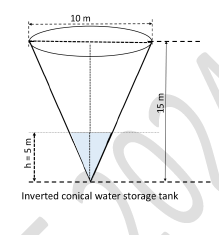
\includegraphics[width=0.5\linewidth]{figs/inverted.png}
  \caption{Inverted conical water tank.}\label{fig:tank}
\end{figure}

\hfill{\brak{\text{GATE MN 2024}}}
% Q45
\item A thermal power plant has an agreement with three mines M1, M2 and M3 to receive Grade 1' coal, in the proportion of 60\%, 25\% and 15\%, respectively. The probabilities that a wagon supplied coal to the plant containing below Grade 1' from mines M1, M2 and M3 are 0.02, 0.03 and 0.04, respectively. On a random check, a sample wagon is found to carry below `Grade 1' coal. The probability that the wagon belongs to mine M1, is \underline{\hspace{1.5cm}}. (round off up to 2 decimals)
\hfill{\brak{\text{GATE MN 2024}}}
% Q46
\item A transportation system for carrying ore from stock pile to railway siding through an ore bin is shown. The time between failure of each conveyor belt follows an exponential distribution with mean time between failure of 700 hours. The system is considered to be a `success' if ore transports from stock pile to siding by any combination of belts. The reliability of the system for 350 hours of continuous successful operation, is \underline{\hspace{1.5cm}}. (round off up to 2 decimals)
\begin{figure}[h!]
\centering
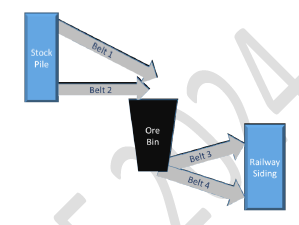
\includegraphics[width=0.5\linewidth]{figs/transportation.PNG}
\caption{Transportation system.}
\label{fig:transport}
\end{figure}
\hfill{\brak{\text{GATE MN 2024}}}
% Q47
\item Polluted air with particulate matter of diameter $50\,\mu\mathrm{m}$ enters with a horizontal velocity of $1.0\ \mathrm{m\,s^{-1}}$ at a height of $0.5\ \mathrm{m}$ from the bottom of a dry settling chamber. The density of the particle is $2000\ \mathrm{kg\,m^{-3}}$ and the dynamic viscosity of air is $1.8\times10^{-5}\ \mathrm{kg\,(m\,s)^{-1}}$. Assume streamline flow, density of air negligible compared to particles, and uniform horizontal velocity of $1.0\ \mathrm{m\,s^{-1}}$ of gas and particles within the chamber. Considering particle settling follows \textit{Stokes'} law, the minimum length (in m) of the chamber required for the particle to settle to the bottom is \underline{\hspace{1.5cm}} (round off to 2 decimals).


\hfill{\brak{\text{GATE MN 2024}}}
% Q48
\item In a tacheometry survey, the readings observed are given (Table~\ref{tab:q48-tacho}).

\begin{center}
  \captionof{table}{Tacheometry observations}\label{tab:q48-tacho}
  \setlength{\tabcolsep}{6pt}
  \renewcommand{\arraystretch}{1.2}
  \begin{tabular}{|c|c|c|c|c|}
    \hline
    \textbf{Instrument Station} & \textbf{Staff Station} &
    \textbf{Bearing of line of sight} & \textbf{Vertical angle} &
    \textbf{Staff readings (m)} \\ \hline
    P & A & $145^\circ$ & $+8^\circ$ & 1.2, 1.7, 2.2 \\ \hline
    P & B & $205^\circ$ & $+3^\circ$ & 0.8, 1.2, 1.6 \\ \hline
  \end{tabular}
\end{center}
 % draws the table exactly here

The additive and multiplying constants of the instrument are $0$ and $100$, respectively.
The length of the line AB in m, is \underline{\hspace{1.5cm}}. \textit{(round off up to 2 decimals)}

\hfill{\brak{\text{GATE MN 2024}}}

% Q49
\item The data obtained from an air sample analysis of an old working in a coal mine are given.\\[0.25em]
$\mathrm{O_2}\ 17.15\%,\ \mathrm{CO_2}\ 3.40\%,\ \mathrm{CH_4}\ 2.20\%,\ \mathrm{N_2}\ 77.25\%.$

\noindent Considering atmospheric air contains\\[0.25em]
$\mathrm{O_2}\ 20.95\%,\ \mathrm{CO_2}\ 0.03\%,\ \mathrm{N_2}\ 79.02\%,$

\noindent the percentage of blackdamp in the old working, is \underline{\hspace{1.5cm}}. \textit{(round off up to 2 decimals)}

\hfill{\brak{\text{GATE MN 2024}}}
% Q50
\item A rectangular face of $2.0\,\mathrm{m}\times2.5\,\mathrm{m}$ is blasted with $20\,\mathrm{kg}$ explosive in a $1000\,\mathrm{m}$ long drive. One kilogram of explosive produces $2200\,\mathrm{cm^3}$ of nitrous fumes. The face is ventilated with a duct, located $10.0\,\mathrm{m}$ away from the face, to dilute the fumes. The quantity of air, in $\mathrm{m^3\,s^{-1}}$, to be circulated for reducing the concentration of nitrous fumes to $5\,\mathrm{ppm}$ within a period of $5$ minutes, is \underline{\hspace{1.5cm}}. \textit{(round off up to 2 decimals)}

\noindent\textit{Use the relation}
\[
t \;=\; 2.303\,\frac{V_m}{Q}\,\log\!\left(\frac{q}{V_m\,c}\right) \;+\; \frac{V - V_m}{Q},
\]
\textit{where } $t=$ time, $V_m=$ volume of the tunnel over which mixing of the gases produced at the face and air delivered by the fan occurs, $c=$ concentration at time $t$, $V=$ volume of tunnel, $Q=$ quantity of air flow, $q=$ total volume of nitrous fumes produced.

\hfill{\brak{\text{GATE MN 2024}}}
% Q51
\item Data for a centrifugal pump discharging water from a sump to the surface are given. Head, m : 180 Discharge rate, m$^3$/hr : 320 Operating hours per day for 270 days in a year : 14 Operating hours per day for remaining 95 days : 20 Overall efficiency of the pumping system : 0.70 Specific weight of mine water, kN/m$^3$ : 10.20 The annual electrical power consumption in GWh, due to pumping operation, is \underline{\hspace{1.5cm}}. (round off up to 2 decimals)
\hfill{\brak{\text{GATE MN 2024}}}
% Q52
\item The root of the function, $f(x) = x^3 - 2x^2 + 3x - 1$ in the interval [0, 1] using bisection method after two iterations, is \underline{\hspace{1.5cm}}. (round off up to 2 decimals)
\hfill{\brak{\text{GATE MN 2024}}}
% Q53
\item A Bord and Pillar panel is developed at a depth of 250 m in a flat coal seam. The vertical stress gradient is 0.027 MPa/m. If the strength of a square pillar is 12.5 MPa, the extraction ratio of the pillar for a safety factor of 1.5, is \underline{\hspace{1.5cm}}. (round off up to 2 decimals)
\hfill{\brak{\text{GATE MN 2024}}}
% Q54
\item A Mohr-Coulomb envelop between shear stress, $\tau$ and normal stress, $\sigma_n$ of a sandstone rock is given as $\tau = 7.5 + 0.84 \sigma_n$ (unit of stresses is MPa) A sandstone sample is tested in triaxial mode with confining pressure of 5.0 MPa. The value of the shear stress, $\tau$ in MPa at the failure, is \underline{\hspace{1.5cm}}. (round off up to 2 decimals)
\hfill{\brak{\text{GATE MN 2024}}}
% Q55
\item A circular tunnel is constructed at a depth of 100 m. The average unit weight of overburden rock is 27.0 kN/m$^3$. If the tangential stress measured at point A located at the horizontal boundary of the tunnel as shown, is 5.0 MPa, the tangential stress at point B in MPa, is \underline{\hspace{1.5cm}}. (round off up to 2 decimals)
\begin{figure}[H] % H = exactly here
  \centering
  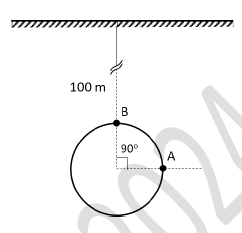
\includegraphics[width=0.5\linewidth]{figs/circular.png}
  \caption{Tunnel section.}\label{fig:tunnel}
\end{figure}

\hfill{\brak{\text{GATE MN 2024}}}
% Q56
\item A mine worker weighing (W) 600 N lifts an object of 100 N as shown. 
The 50\% body weight is applied downward through point A and a force $F_E$ is produced parallel to $x$ axis by the contraction of erector spinae muscle during lifting. 
The lumbar disc, L (shown by red box) acts as a smooth hinge and keeps the upper body in static equilibrium. 
Ignore all other forces in the body. 
The magnitude of the resultant of the reaction forces, in N at the lumbar disc, is \underline{\hspace{1.5cm}}. (round off up to 2 decimals)

\par\noindent
\begin{minipage}{\linewidth}
  \centering
  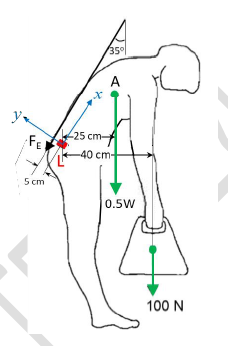
\includegraphics[width=0.5\linewidth]{figs/worker.png}% check exact filename/case
  \captionof{figure}{Lifting posture.}\label{fig:lift}
\end{minipage}

\hfill{\brak{\text{GATE MN 2024}}}

\hfill{\brak{\text{GATE MN 2024}}}
% Q57
\item A solid ball of mass 10 kg is subjected to forces as shown. The magnitude of the acceleration in m/s$^2$, is \underline{\hspace{1.5cm}}. (round off up to 2 decimals)
\begin{figure}[h!]
\centering
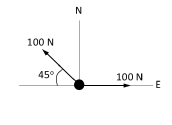
\includegraphics[width=0.5\linewidth]{figs/forces.png}
\caption{Forces on ball.}
\label{fig:ball}
\end{figure}
\hfill{\brak{\text{GATE MN 2024}}}
\newpage
% Q58
\item In an open pit mine, the mineral inventory, prices, costs and capacities are given
(Table~\ref{tab:q58-inv}).

\begin{center}
  \captionof{table}{Mineral inventory}\label{tab:q58-inv}
  \begin{tabular}{|c|c|}
    \hline
    \textbf{Grade interval} & \textbf{Tonnage (in million tonne)} \\ \hline
    $0 < \mathrm{Cu}\% \le 0.3$   & 0 \\ \hline
    $0.3 < \mathrm{Cu}\% \le 0.4$ & 5 \\ \hline
    $0.4 < \mathrm{Cu}\% \le 0.5$ & 5 \\ \hline
    $0.5 < \mathrm{Cu}\% \le 0.6$ & 5 \\ \hline
    $0.6 < \mathrm{Cu}\% \le 0.7$ & 5 \\ \hline
    $0.7 < \mathrm{Cu}\% \le 0.8$ & 5 \\ \hline
    $0.8 < \mathrm{Cu}\%$         & 0 \\ \hline
  \end{tabular}
\end{center}
 % inserts the table exactly here

\noindent
\begin{tabular}{@{}l l@{}}
Concentrating cost &: INR 3,200/tonne of ore milled \\
Smelting \& refinery cost &: INR 10,000/tonne of copper metal \\
Selling price &: INR 6,50,000/tonne of copper metal \\
Overall recovery &: 100\% \\
Maximum production capacity &: 5 million tonne/annum \\
\end{tabular}

\medskip
The mine is operating at 5 million tonne in a year. Considering mining capacity as the only
constraint, Lane's algorithm (based on profit maximization) is used for determining mill
cut-off grade. The total amount of copper produced in million tonne, in the life of the pit, is
\underline{\hspace{1.5cm}}. \textit{(round off up to 2 decimals)}

\hfill{\brak{\text{GATE MN 2024}}}
% Q59
\item A longitudinal section of a mined out stope block in a copper mine is shown by the shaded portion. For a uniform thickness of the stope block, the percentage of ore recovery, is \underline{\hspace{1.5cm}}. (round off up to 2 decimals)
\begin{figure}[h!]
\centering
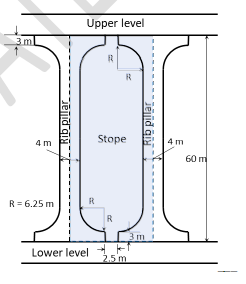
\includegraphics[width=0.5\linewidth]{figs/section.png}
\caption{Stope section.}
\label{fig:stope}
\end{figure}
\hfill{\brak{\text{GATE MN 2024}}}
% Q60
\item The real rate of return from a mining project is $14\%$. If the inflation rate over the entire life of the mine is $5.5\%$, then the nominal rate of return, in \%, is \underline{\hspace{1.5cm}}. \textit{(round off up to 2 decimals)}

\hfill{\brak{\text{GATE MN 2024}}}
% Q61
% --- Main file snippet ---
\item In an opencast coal mine, blast vibrations are measured at two locations, A and B
simultaneously for a maximum charge per delay $(Q)$ of $1200\ \mathrm{kg}$ as given
(Table~\ref{tab:q61-ppv}).

\begin{center}
  \captionof{table}{Vibration data for scaled-distance relation}\label{tab:q61-ppv}
  \begin{tabular}{|c|c|c|}
    \hline
    \textbf{Location} & \textbf{Distance from the blast face, $D$ (m)} & \textbf{PPV (mm/s)} \\ \hline
    A & 100 & 112.5 \\ \hline
    B & 300 & 20.3 \\ \hline
  \end{tabular}
\end{center}
 % draws the table exactly here

Assume the relation
\[
\mathrm{PPV}=K\left(\frac{D}{\sqrt{Q}}\right)^{-\beta}
\]
where, $K$ and $\beta$ are site constants. The PPV in mm/s, at a distance of
$200\ \mathrm{m}$ from the blast face, is \underline{\hspace{1.5cm}}.
\textit{(round off up to 2 decimals)}

\hfill{\brak{\text{GATE MN 2024}}}
% Q62
\item A 35.0 kW motor transmits power to a pulley of 600 mm diameter, which rotates at 400 rpm to drive a flat belt. The tension in the tight side is 2.5 times of the slack side. Neglect all transmission losses. If the maximum allowable tension is 8.0 N per mm of belt width, then the minimum width of the belt in mm, is \underline{\hspace{1.5cm}}. (round off up to 2 decimals)
\hfill{\brak{\text{GATE MN 2024}}}
% Q63
\item A 1.2 m diameter drum winding system is shown. One of the winding ropes will be replaced for the manwinding cage.
\begin{figure}[h!]
\centering
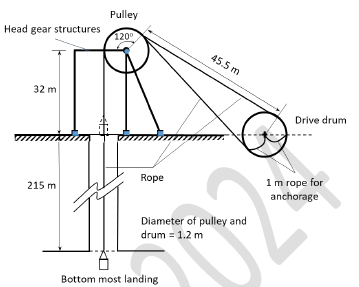
\includegraphics[width=0.5\linewidth]{figs/winding.png}
\caption{Winding system.}
\label{fig:winding}
\end{figure}
Consider the following:

1) A new rope is recapped once at least in every 6 months and a length of 2 m including existing capping is to be cut off from the rope before recapping.\\[0.5em]
2) The maximum life of a rope is 3.5 years and at least 2 rounds of rope should remain on the drum while the descending cage lands at the bottommost landing point.\\[0.5em]
3) No overwinding will take place during the maximum life of the new rope.\\[0.5em]
Neglecting the impact of fleet angle on the length of the rope, the minimum length, in m, of new winding rope is \underline{\hspace{1.5cm}}. (round off up to 2 decimals)

\hfill{\brak{\text{GATE MN 2024}}}
% Q64
\item For a continuous miner (CM) panel, the following data are given.

\noindent\textbf{Data related to CM}
\begin{center}
\begin{tabular}{@{}p{0.58\linewidth}@{\hspace{0.6em}: }p{0.32\linewidth}@{}}
Dimension of a working face & $5.0\,\mathrm{m}$ (width) $\times$ $3.0\,\mathrm{m}$ (height) \\
Web depth, m & $0.6$ \\
Time for one web cut up to full height, min & $9$ \\
\end{tabular}
\end{center}

\noindent\textbf{Data related to shuttle car}
\begin{center}
\begin{tabular}{@{}p{0.58\linewidth}@{\hspace{0.6em}: }p{0.32\linewidth}@{}}
Bucket capacity of shuttle car, tonne & $10$ \\
Fill factor & $0.9$ \\
Number of cars & $2$ \\
Cycle time of each car including loading, travel and unloading, min & $6$ \\
\end{tabular}
\end{center}

\noindent Assume, unit weight of coal is $1.4\ \text{tonne/m}^3$ and its swell factor is $1.2$. Consider $6$ working hours per shift.

\noindent The non-working time in min, in working hours per shuttle car to dispatch all coal cut by the CM, is \underline{\hspace{1.5cm}}. \textit{(round off up to 2 decimals)}

\hfill{\brak{\text{GATE MN 2024}}}
% Q65
\item In a development coal face, 12 holes are drilled and charged with explosive. 
Holes are initiated with electric delay detonators connected in series. 
The length of a detonator lead wire is $1.5\,\mathrm{m}$. 
The length of the blasting cable is $120\,\mathrm{m}$.

\noindent\textbf{Data are as given:}
\begin{center}
\begin{tabular}{@{}p{0.58\linewidth}@{\hspace{0.6em}: }p{0.32\linewidth}@{}}
Resistance of each detonator & $1.48\,\Omega$ \\
Resistance of lead wire & $0.04\,\Omega/\mathrm{m}$ \\
Resistance of one wire of the blasting cable & $0.009\,\Omega/\mathrm{m}$ \\
\end{tabular}
\end{center}

\noindent The total resistance of the circuit, in $\Omega$, is \underline{\hspace{1.5cm}}. \textit{(round off up to 2 decimals)}

\hfill{\brak{\text{GATE MN 2024}}}
\vspace{2em}
\begin{center}
\textbf{\textsc{END OF THE QUESTION PAPER}}
\end{center}
\end{enumerate}
\end{document}
